\documentclass[Space_Shuttle_Ultra_Manual.tex]{subfiles} 
\begin{document}

\section{UPPER STAGES}
\begin{multicols*}{2}
\label{sec:upper-stages}
\renewcommand{\cfttoctitlefont}{\bf}
\localtableofcontents
\noindent
\\
Currently SSU supports the 2 biggest and more powerful Space Shuttle upper stages$\colon$ the Centaur and the Inertial Upper Stage. These 2 upper stages allow the Space Shuttle Ultra add-on to launch payloads to anywhere from GEO to the depths of the Solar System.
\end{multicols*}

\subsection{Centaur}
\begin{multicols*}{2}
\renewcommand{\cfttoctitlefont}{\bf}
\localtableofcontents
\subsubsection{Description}
\noindent
In the 1980s, NASA modified the Centaur upper stage with the intent to use it aboard the Space Shuttle to increase the payload capability of space probes and GEO satellites.\\
%In the 1980s, NASA modified the Centaur upper stage with the intent to use it aboard the Space Shuttle, thus allowing heavy payloads to be launched to anywhere from GEO to the depths of the Solar System.

\begin{figure}[H]
	\centering
	\captionsetup{justification=centering}
  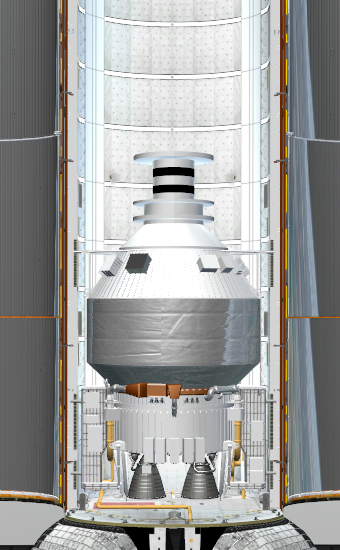
\includegraphics[width=0.99\hsize]{centaurG.png}
  \caption{Centaur G installed in the payload bay with SSU\_DemoSat}
  \label{fig:centaurG}
\end{figure}

Two versions were developed$\colon$ the Centaur G version was primarily for GEO satellite deployment missions, and the larger, more powerful Centaur G Prime for interplanetary payloads. In the aftermath of the Challenger accident, the Centaur was no longer considered safe enough to be used by the Space Shuttle, and so it was abandoned.
\\
Thrust is provided by 2 RL-10 engines, and the Attitude Control System (ACS) allows 3-axis control of the stage, and also translation in the +Z direction (forward).

\begin{figure}[H]
	\centering
	\captionsetup{justification=centering}
  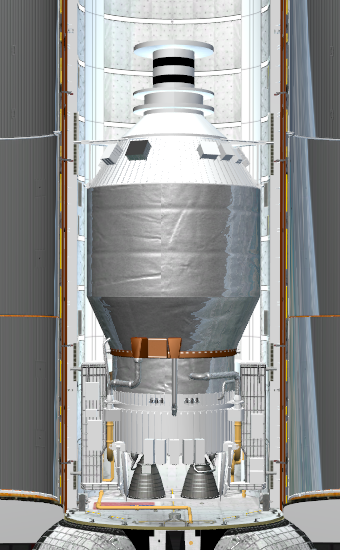
\includegraphics[width=0.99\hsize]{centaurGP.png}
  \caption{Centaur G Prime installed in the payload bay with SSU\_DemoSat}
  \label{fig:centaurGP}
\end{figure}

\subsubsection{Performance}
\begin{figure}[H]
	\centering
	\captionsetup{justification=centering}
  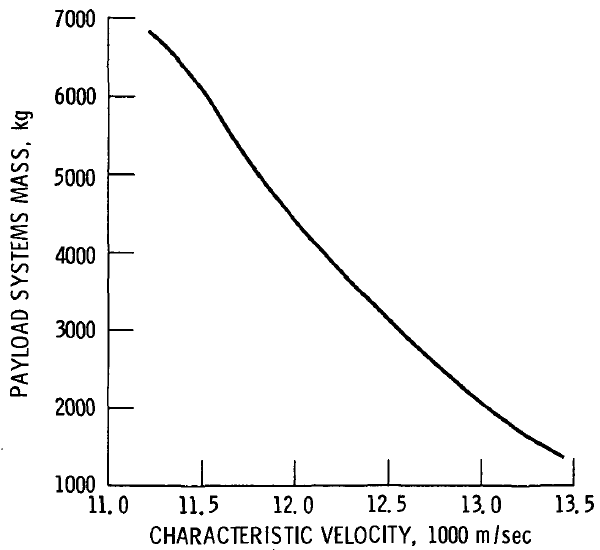
\includegraphics[width=0.99\hsize]{Gpayload.png}
  \caption{Centaur G payload capability for an Earth-escape trajectory}
  \label{fig:Gpayload}
\end{figure}
\noindent
Although the Centaur G is suited for GEO satellite missions, it is also capable of launching spacecraft into Earth-escape trajectories. A plot of payload mass versus characteristic velocity achievable with the Centaur G in shown in figure \ref{fig:Gpayload}.

\begin{figure}[H]
	\centering
	\captionsetup{justification=centering}
  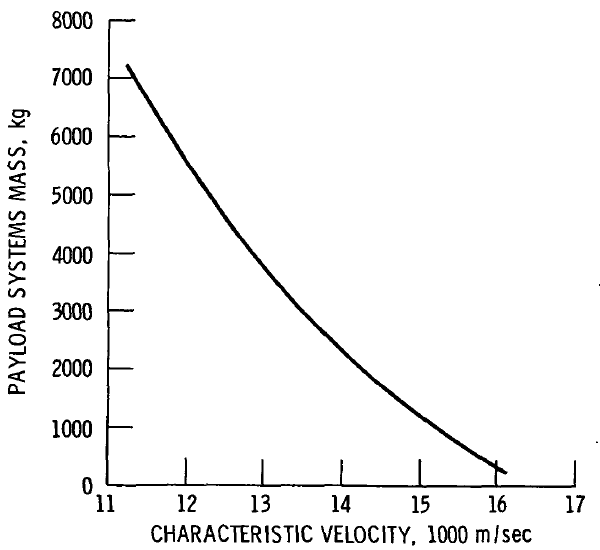
\includegraphics[width=0.99\hsize]{GPpayload.png}
  \caption{Centaur G Prime payload capability for an Earth-escape trajectory}
  \label{fig:GPpayload}
\end{figure}
\noindent
The greater propellant capability of the Centaur G Prime gives it the performance needed to launch heavy spacecraft to other planets. A plot of payload mass versus characteristic velocity achievable with the Centaur G Prime in shown in figure \ref{fig:GPpayload}.

\begin{figure*}[ht]
  \centering
  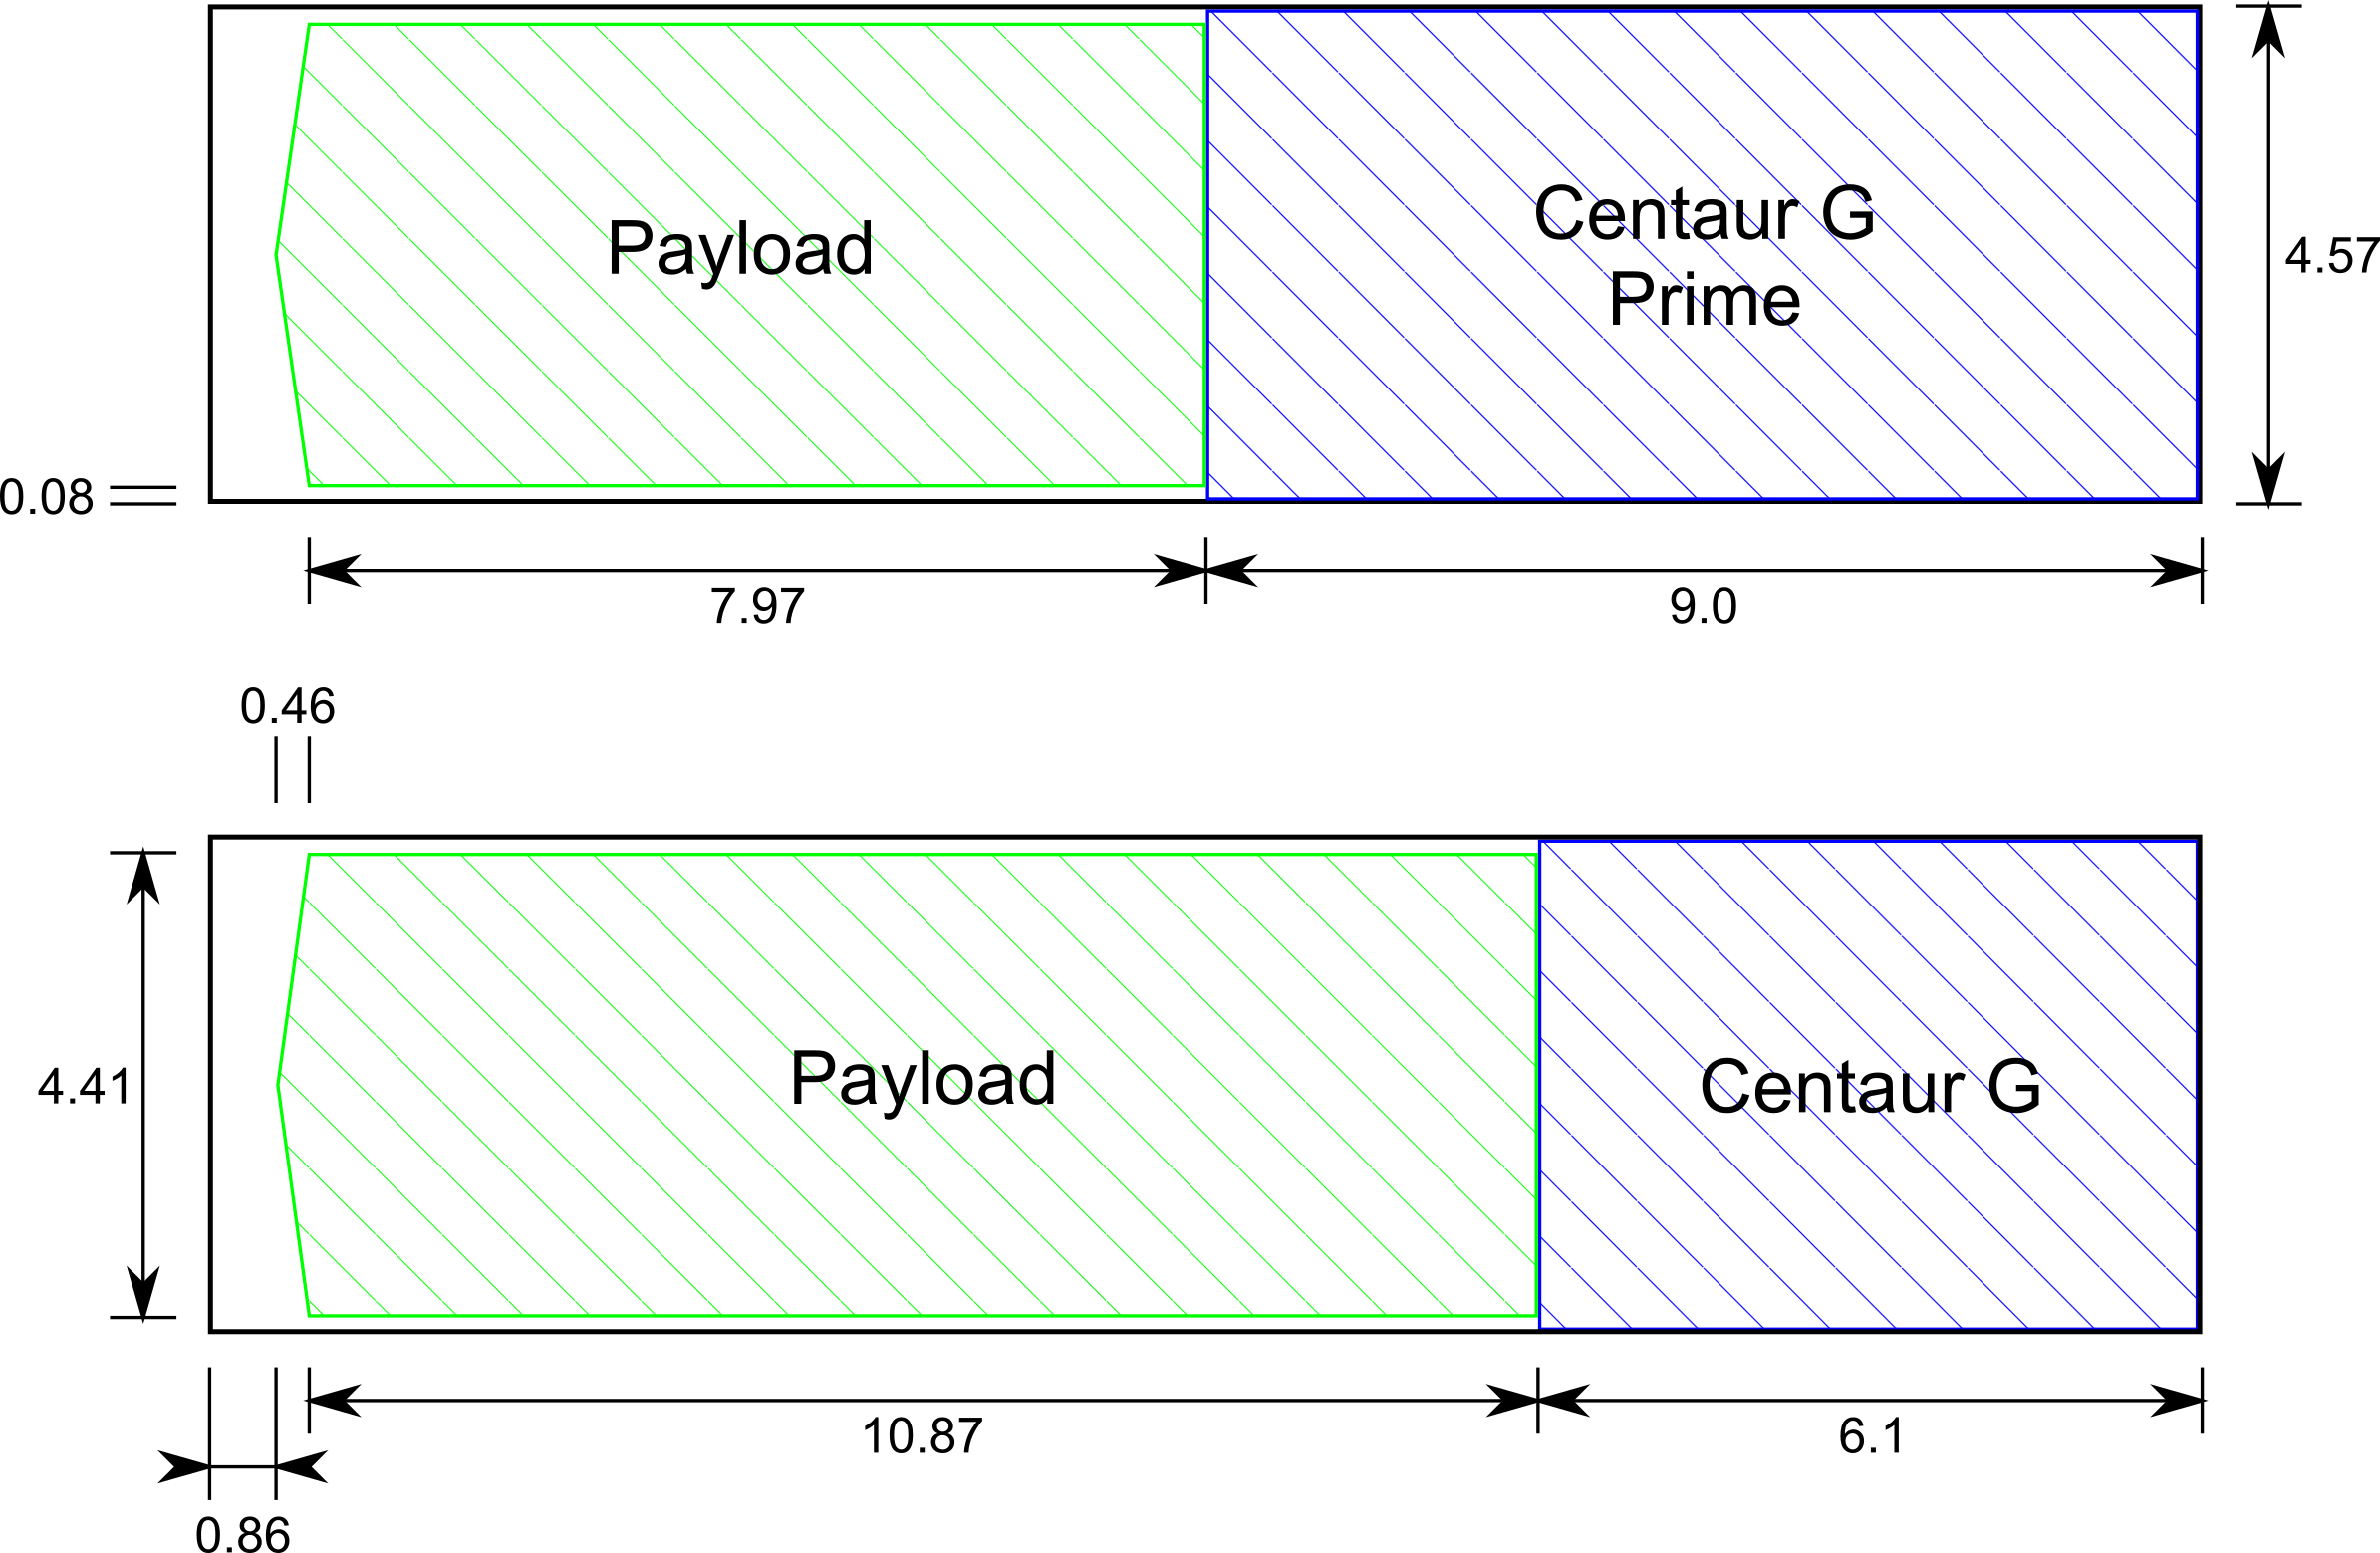
\includegraphics[width=1\textwidth]{payload_volume_centaur.png}
  \caption{Centaur G and G Prime payload envelope (dimensions in meters)}
  \label{fig:payload_volume_centaur}
\end{figure*}
\noindent
Figure \ref{fig:payload_volume_centaur} shows the allowable payload envelope for both Centaur versions. The higher performance of the Centaur G Prime comes at a cost in allowable payload volume.

\subsubsection{Centaur Integrated Support Structure}
The Centaur Integrated Support Structure (CISS) is the interface between the Centaur stage and the orbiter vehicle. Before Centaur deployment, the CISS provides the Centaur with fluid connections for propellant loading and dumping, electrical power and communications, and serves to secure it inside the payload bay. The CISS has a tilt table, to which the Centaur is attached, allowing it to be raised above the payload bay for deployment.

\subsubsection{Deployment}
The deployment sequence is similar for both Centaur versions, and is controlled by panel L12U. A checklist is available in section \ref{sec:flight-data-files}.
\\
Inhibits are placed on the operation of the ACS and of the RL-10 engines, as to protect the orbiter vehicle. At deployment, timers are started to remove those inhibits. The status of those timers is displayed in the SSU\_Centaur MFD (Ctrl+T), as well as the remaining ACS propellant.

\subsubsection{Autonomous flight control}
After separation from the CISS and the engine inhibits have been removed, the Centaur is controlled by using the standard Orbiter keys. The ''+'' key is used to initiate the start sequence for the RL-10 engines. The start sequence is a 270-second chill-down of the RL-10s concurrent with a propellant settling burn by the forward-thrusting ACS. After the chill-down is complete, RL-10 ignition occurs automatically. After the start sequence is initiated, the time remaining until ignition is shown in the SSU\_Centaur MFD. Currently there are no restrictions on the number of times the RL-10 engines can be started. The ''-'' key is used to shutdown the engines once the desired $\Delta$V has been achieved. During RL-10 burns the attitude in completely controlled by gimballing the engine nozzles.
\\
\\
\WARNING{Engine gimballing is much more powerful than the ACS, so it must be used carefully so the stage is not put into a tumble that might be impossible for the ACS to correct after the burn.}
\\
\\
Manual command for the engine gimbal is available and when there is no user input, the rates will be automatically nulled. After all the necessary burns are performed, payload separation is done by pressing the ''Ctrl+J'' key combination.

\subsubsection{Payload Interface}
The connection between the Centaur and its payload is done using a payload adapter. Its exclusive purpose is to interface the payload with the Centaur and is considered a part of the payload, even though on payload deployment the adapter remains with the Centaur.\\
The payload adapter is specified in the Centaur vessel section of the scenario file (section \ref{sec:scenario-files}).
For Centaur payload developers, the payload adapter must be 2.74 meters in diameter at the Centaur end, to correctly interface with the stage. The payload adapter can be a solid tapered cone as shown in figures \ref{fig:centaurG} and \ref{fig:centaurGP} or a grid structure. SSU includes a demonstration payload adapter for interfacing the Centaur with SSU\_DemoSat.

\end{multicols*}
\newpage

\subsection{Inertial Upper Stage}
\begin{multicols*}{2}
\renewcommand{\cfttoctitlefont}{\bf}
\localtableofcontents
\subsubsection{Description}
\noindent
The Inertial Upper Stage, or IUS, is a 2-stage solid propellant vehicle used in several Space Shuttle missions to boost satellites into GEO and space probes into Earth escape trajectories.
\\
\begin{figure}[H]
	\centering
	\captionsetup{justification=centering}
  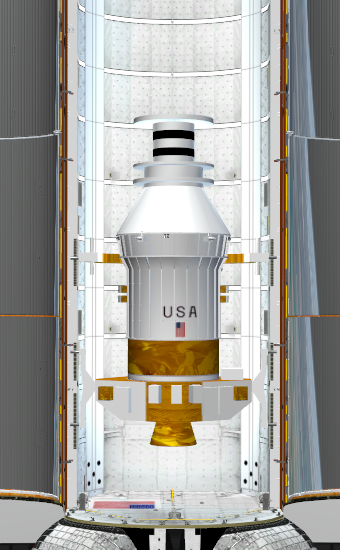
\includegraphics[width=0.99\hsize]{ius.png}
  \caption{Inertial Upper Stage installed in the payload bay with SSU\_DemoSat}
  \label{fig:ius}
\end{figure}
\noindent
Thrust is provided by one Solid Rocket Motor (SRM) in each stage, and the Reaction Control System (RCS) allows 3-axis control of the stage, and also translation in the +Z direction (forward).\\

\subsubsection{Configuration}
\noindent
The IUS can be installed in the payload bay in 2 possible positions: the forward position or the aft position (for large payloads). The position choice is defined in the mission file (section \ref{sec:mission-files}).\\
The standard IUS configuration features 2 RCS tanks each with 55Kg of propellant. An additional tank can be used, for a total of 3, or only one tank can be used to reduce mass. In addition to the standard 2 omni-directional antennas in the $2^{nd}$ stage, a further 2 can be added, for a total of 4. Due to the nature of the solid propellant motors, fine control of the $\Delta$V is impossible during the burn, so the propellant quantity must be carefully set. Both SRMs have the capability to be offloaded up to 50\%.\\
The number of RCS tanks, omni-directional antennas and SRM propellant offload quantity are controlled by scenario file parameters (section \ref{sec:scenario-files}).

\subsubsection{Performance}
\begin{figure}[H]
	\centering
	\captionsetup{justification=centering}
  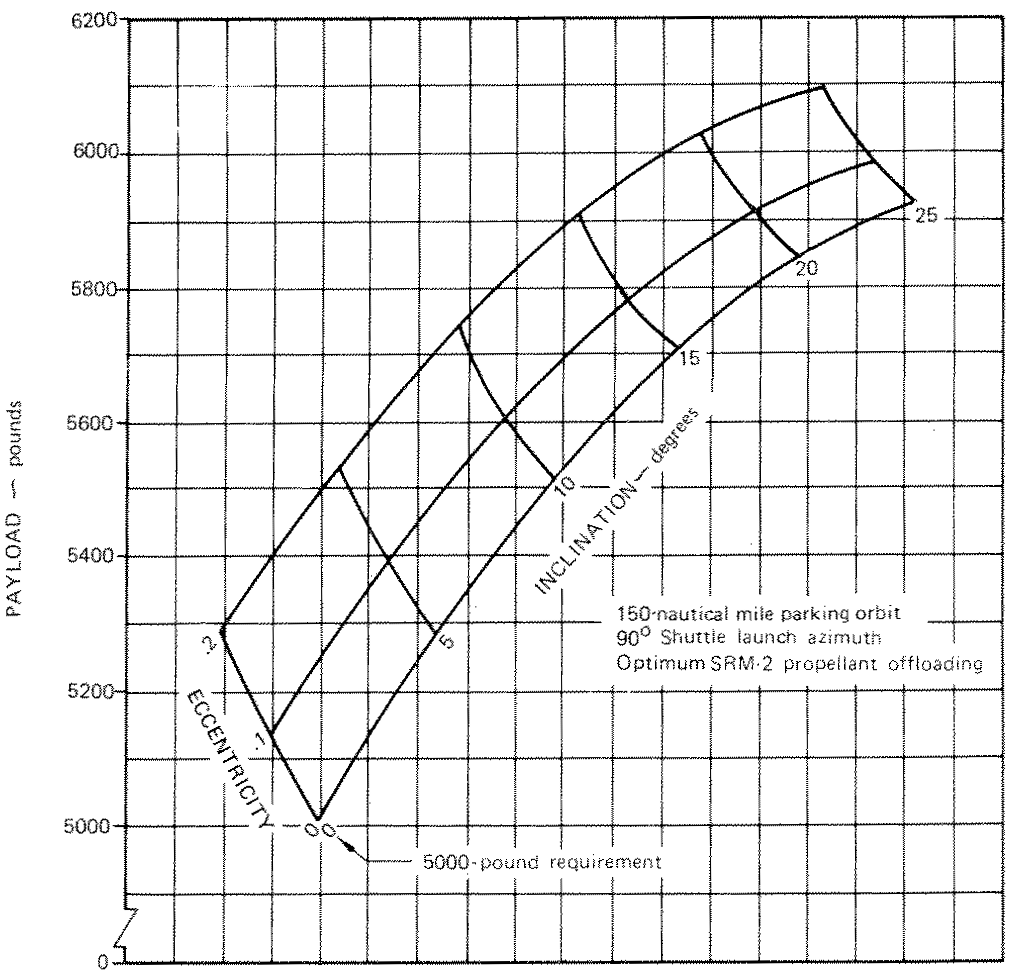
\includegraphics[width=0.99\hsize]{IUSpayloadGEO.png}
  \caption{IUS payload capability to GEO}
  \label{fig:IUSpayloadGEO}
\end{figure}
\noindent
Specially suited for GEO missions, the IUS was designed to insert a 5000-pound (2268 Kg) payload into geostationary orbit. It can however launch heavier payloads at the expense of final orbit eccentricity and/or inclination. The relationship between payload mass and the corresponding achievable orbital parameters for a GEO mission is shown in figure \ref{fig:IUSpayloadGEO}.\\

\begin{figure}[H]
	\centering
	\captionsetup{justification=centering}
  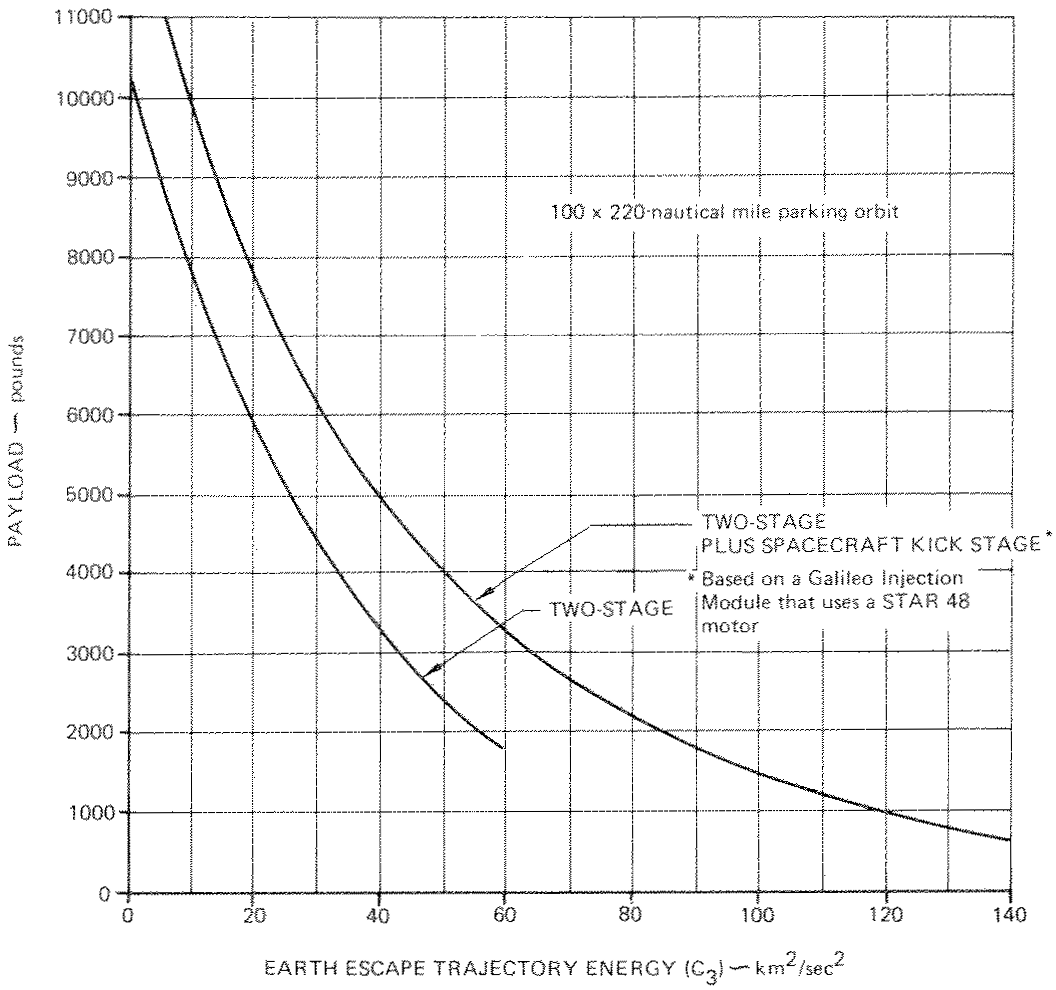
\includegraphics[width=0.99\hsize]{IUSpayloadC3.png}
  \caption{IUS payload capability for an Earth-escape trajectory}
  \label{fig:IUSpayloadC3}
\end{figure}
\noindent
Although designed for Earth-orbit missions, the IUS can also inject spacecrafts into low-energy Earth-escape trajectories. More capability can be obtained by including an additional stage in the spacecraft. The payload capability of the IUS versus C3 energy is presented in figure \ref{fig:IUSpayloadC3}.

\begin{figure*}[t!]
  \centering
  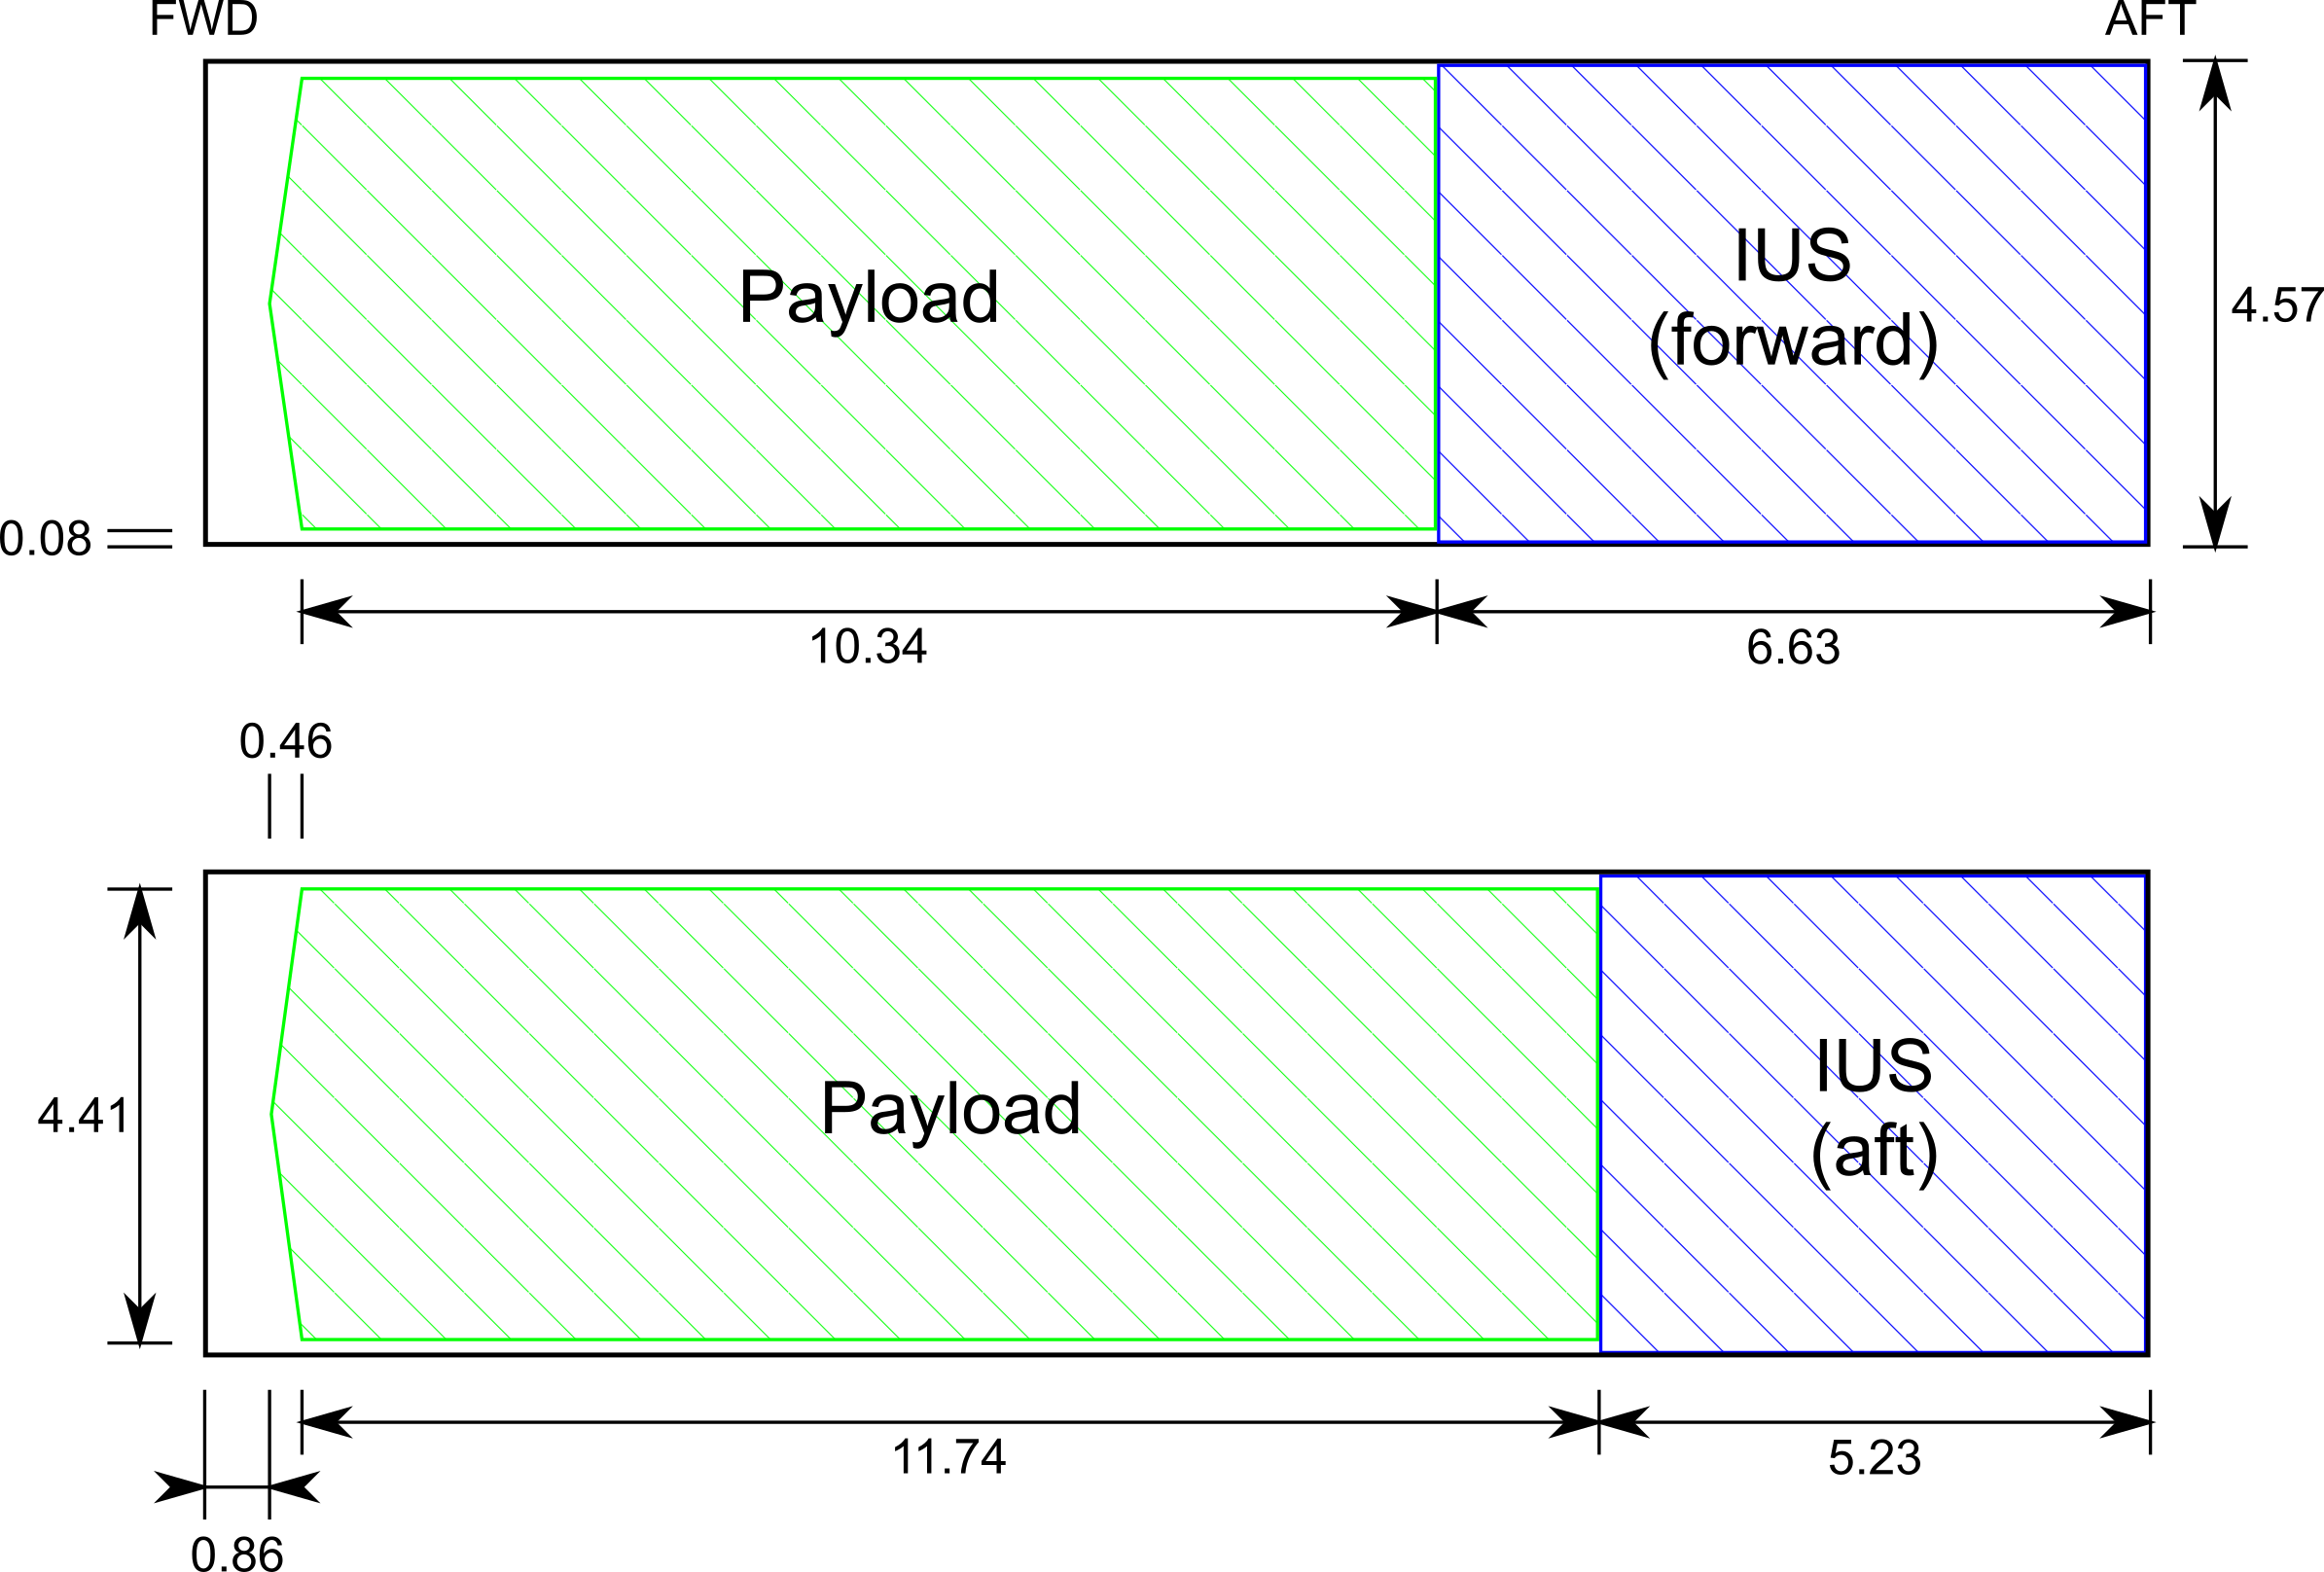
\includegraphics[width=1\textwidth]{payload_volume_ius.png}
  \caption{IUS payload envelope (dimensions in meters)}
  \label{fig:payload_volume_ius}
\end{figure*}
\noindent
Figure \ref{fig:payload_volume_ius} shows the allowable payload envelope for both IUS positions. While the aft IUS position allows a payload with greater volume to be carried, it should only be used when necessary due to orbiter vehicle c.g. concerns.

\subsubsection{Airborne Support Equipment}
The Airborne Support Equipment (ASE) is the interface between the IUS and the orbiter vehicle. Before IUS deployment, the ASE provides the IUS with electrical power and communications, and serves to secure it inside the payload bay. The ASE has a tilt table, to which the IUS is attached, allowing it to be raised above the payload bay for deployment. The ASE also has a boom-mounted IUS umbilical, that must be released before IUS deployment.

\subsubsection{Deployment}
The IUS deployment sequence is controlled by panel L10.
\\
TODO
\\
Inhibits are placed on the operation of the RCS and of the $1^{st}$ stage motor, as to protect the orbiter vehicle. At deployment, timers are started to remove those inhibits. The status of those timers is displayed in the SSU\_IUS MFD (Ctrl+T), as well as the remaining RCS propellant.

\subsubsection{Autonomous flight control}
After separation from the ASE and the engine inhibits have been removed, the IUS is controlled by using the standard Orbiter keys. The ''+'' key is used to ignite the SRMs. During SRM burns the attitude in the pitch and yaw axis is controlled by gimballing the engine nozzle, while roll remains under RCS control.
\\
\\
\WARNING{Engine gimballing is much more powerful than the RCS, so it must be used carefully so the stage is not put into a tumble that might be impossible for the RCS to correct after the burn.}
\\
\\
Manual command for the engine gimbal is available and when there is no user input, the rates will be automatically nulled. Once ignited, the SRMs will burn to depletion.\\
After $1^{st}$ stage burnout, its separation is done by pressing the ''Ctrl+G'' key combination. After $1^{st}$ stage separation, the Extendable Exit Cone in the $2^{nd}$ stage will automatically deploy.\\
At the end of each SRM burn, the RCS can be used for velocity fine tuning.\\
After all the burns are performed, payload separation is done by pressing the ''Ctrl+J'' key combination.

\subsubsection{Payload Interface}
The connection between the IUS and its payload is done using a payload adapter. Its exclusive purpose is to interface the payload with the IUS and is considered a part of the payload, even though on payload deployment the adapter remains with the IUS.\\
The payload adapter is specified in the IUS vessel section of the scenario file (section \ref{sec:scenario-files}).
For IUS payload developers, the payload adapter must be 2.89 meters in diameter at the IUS end, to correctly interface with the stage. The payload adapter can be a solid tapered cone as shown in figure \ref{fig:ius} or a grid structure. SSU includes a demonstration payload adapter for interfacing the IUS with SSU\_DemoSat.\\

\end{multicols*}
\end{document}